\documentclass[11pt]{article}
\usepackage[a4paper, total={7in, 10in}]{geometry}
\usepackage{amsmath}
\usepackage{graphicx}
\usepackage{hyperref}
\graphicspath{ {.} }
\usepackage[font=small,labelfont=bf]{caption} % Required for specifying captions to tables and figures
\usepackage[T1]{fontenc}
\usepackage[utf8]{inputenc}


\title{Discrete Algorithms - Max Flow algorithms}
\author{Mateusz Pełechaty}
\date{22 June 2023}%
\begin{document}
\maketitle
\section{Exercise. Edmund Karp on HyperCube}
Goal of this exercise was to 
\begin{enumerate}
    \item create graph of hypercube with random residual capacities from given range
    \item find max flow from $(0)^n$ to $(1)^n$
    \item conduct tests for several k where k is amount of dimensions of cube.
\end{enumerate} 
\subsection{Plots}

\begin{figure}[h!]
    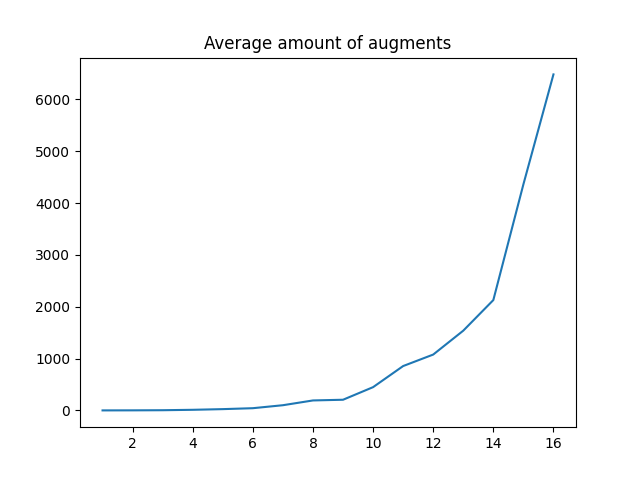
\includegraphics{plots/augments.png} 
\end{figure}

\begin{figure}[h!]
    \includegraphics*{plots/flow.png}
\end{figure}
\begin{figure}[h!]
    \includegraphics*{plots/time.png}
\end{figure} 

\section{Exercise. Edmund Karp. Maximum Bipartite Matching}
In this exercise we should find maximum matching for bipartite graph.
We will use edmund karp algorithm for it, by reducing maximum bipartite matching to max flow problem through adding source with edges to all vertices from first set and sink with edges from every vertice from set2 towards sink. \\
  
\subsection{Plots}
\begin{figure}[h!]
    \includegraphics*{zad2_plots/max_flow.png}
\end{figure} 

\begin{figure}[h!]
    \includegraphics*{zad2_plots/time.png}
\end{figure}
\end{document} 

